\chapter{Методы решения задачи классификации изображений растения}
\section{Методы классификации на основе ручного извлечения признаков}
В данном разделе рассматриваются методы классификации изображений растений, основанные на ручном извлечении признаков и последующем применении алгоритмов машинного обучения. 
\textbf{Локальные бинарные паттерны}
Для заданного текстурного изображения LBP-код с параметрами $P$ и $R$, где $P$ равномерно расположенных пикселей выбираются на окружности радиуса $R$ относительно центрального пикселя, вычисляется для каждого пикселя изображения следующим образом:
\begin{equation}
	\mathrm{LBP}_{P,R} = \sum_{i=1}^{P} S \cdot 2^{i-1},
\end{equation}
где функция $S$ определяется как
\begin{equation}
	S =
	\begin{cases}
		1, & \text{если } (G_i - G_c) \geqslant 0, \\
		0, & \text{в противном случае}.
	\end{cases}
\end{equation}

Здесь $G_c$ и $G_i$ обозначают значения яркости центрального пикселя и соответствующего соседнего пикселя соответственно.

\clearpage
Пример взятия пикселей с различными заданными P, R приведён на рисунке~\ref{lbp_radious}.

\begin{figure}[h]
	\centering
	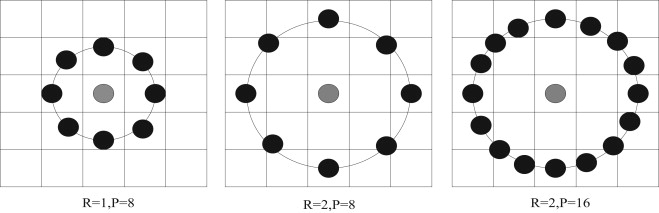
\includegraphics[width=\linewidth]{inc/img/lbp_radious.jpg}
	\caption{Схема выбора соседних пикселей в дескрипторе LBP для различных значений параметров $(P, R)$}
	\label{lbp_radious}
\end{figure}

В результате каждому пикселю изображения сопоставляется LBP-код, принимающий значения в диапазоне $[0, 2^{P} - 1]$. Далее всё изображение представляется в виде гистограммы, построенной по частотам появления LBP-кодов, вычисленных для всех пикселей изображения.

Базовый оператор LBP основан на жёстком пороговом сравнении, которое зависит от разности значений яркости центрального пикселя и соседнего пикселя. При этом возможно, что различные локальные пространственные структуры будут иметь одинаковый LBP-код, несмотря на различия в их геометрической организации. Это ограничивает дискриминативную способность базового LBP-дескриптора при различении сложных структурных паттернов~\cite{ref1000}.

Пример вычисления LBP-кода приведён на рисунке~\ref{lbp_example}
\begin{figure}[h]
	\centering
	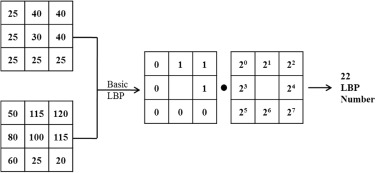
\includegraphics[width=\linewidth]{inc/img/lbp_example.jpg}
	\caption{Пример вычисления LBP-кода пикселя}
	\label{lbp_example}
\end{figure}
\clearpage

\textbf{Гистограмма ориентированных градиентов}

Метод базируется на анализе распределения направлений локальных градиентов яркости в плотной сетке и относится к классу плотных дескрипторов изображений.

Основная идея заключается в том, что локальный внешний вид и форма объекта могут быть эффективно охарактеризованы распределением направлений градиентов или границ, даже без точного знания их пространственного положения. На практике это реализуется путём разбиения изображения на небольшие пространственные области (ячейки), внутри которых накапливаются одномерные гистограммы направлений градиентов или ориентаций границ по всем пикселям соответствующей ячейки. Полученные значения гистограмм образуют вектор признаков.

Для повышения устойчивости к изменениям освещения, затенению и локальным изменениям контраста выполняется нормализация локальных откликов. Для этого энергия гистограмм аккумулируется в более крупных пространственных областях (блоках), после чего значения гистограмм всех ячеек, входящих в блок, нормализуются. Нормализованные блоки гистограмм образуют дескрипторы HOG.

Несмотря на успех разреженных признаков, таких как ключевые точки, плотное представление изображения в виде HOG-дескрипторов сохраняет высокую информативность и простоту, что делает его эффективным средством описания формы объектов.

Дескрипторы HOG обладают рядом преимуществ. Они эффективно захватывают структуру границ и градиентов, характерную для локальной формы объекта, и при этом обеспечивают контролируемую инвариантность к локальным геометрическим и фотометрическим преобразованиям. Небольшие смещения и повороты оказывают незначительное влияние на описание, если их масштаб меньше размера пространственных ячеек или угловых интервалов гистограммы.~\cite{ref1001}

Основные этапы реализации дескриптора HOG включают:
\begin{itemize}[label=---]
	\item вычисление градиентов изображения;
	\item построение гистограмм ориентаций для заданных областей;
	\item нормализацию гистограмм внутри сформированных групп областей.
\end{itemize}

Вычисление градиентов.
На первом этапе цветные текстурные изображения преобразуются в изображения в градациях серого. Горизонтальный градиент $f_a$ и вертикальный градиент $f_b$ вычисляются с использованием дифференцирующих масок для изображения в градациях серого. Применение более сложных масок снижает производительность системы, поэтому используется простая дифференцирующая маска. Горизонтальный $f_a$ и вертикальный $f_b$ градиенты изображения вычисляются следующим образом:
\begin{equation}
	f_a(a,b) = I(a+1,b) - I(a-1,b),
\end{equation}
\begin{equation}
	f_b(a,b) = I(a,b+1) - I(a,b-1),
\end{equation}
где $I(a,b)$ представляет значение интенсивности пикселя в точке $(a,b)$.

Построение гистограмм ориентаций.
С использованием горизонтального $f_a$ и вертикального $f_b$ градиентов изображения вычисляются величина градиента $m$ и ориентация градиента $\theta$ следующим образом:
\begin{equation}
	m(a,b) = \sqrt{f_a(a,b)^2 + f_b(a,b)^2},
\end{equation}
\begin{equation}
	\theta(a,b) = \tan^{-1}\left(\frac{f_b(a,b)}{f_a(a,b)}\right).
\end{equation}

Направленная гистограмма градиентов.
На практике ориентации градиента, меньшие нуля, суммируются с $180^\circ$, поскольку требуемые значения направлений должны быть немаркированными. Соответственно, немаркированные ориентации градиентов нового изображения вычисляются следующим образом:
\begin{equation}
	\tilde{\theta}(a,b) =
	\begin{cases}
		\theta(a,b) + \pi, & \text{если } \theta(a,b) < 0, \\
		\theta(a,b), & \text{в противном случае}.
	\end{cases}
\end{equation}

После вычисления ориентаций градиентов изображение разбивается на ячейки фиксированного размера $[u \times v]$ пикселей. Угол ориентации $\tilde{\theta}(a,b)$ распределяется по соответствующему угловому интервалу для формирования гистограммы ориентаций каждой ячейки. Гистограмма ориентаций формируется путём равномерного разбиения диапазона $0^\circ$--$180^\circ$

Нормализация по блокам.
Блочная нормализация отображает гистограммы ориентаций для каждой ячейки с вычитанием больших блоков размером $[n \times m]$. Поскольку каждая ячейка содержит $k$ ориентаций, размер вектора признаков для каждого блока составляет $[n \times m \times k]$. Вектор признаков $\mathbf{v}$ представляет ненормализованную гистограмму в точке $(i,j)$ блока $p(i,j)$. Нормализация вектора признаков выполняется с использованием $L_2$-нормы следующим образом
\begin{equation}
	\mathbf{v}' = \frac{\mathbf{v}}{\sqrt{\|\mathbf{v}\|^2 + \varepsilon}}
\end{equation}
где $\varepsilon$~---~малая нормализующая константа, используемая для предотвращения деления на ноль.

Иллюстрация получения гистограммы для ячейки представлен на изображении~\ref{hog_example}

\begin{figure}[h]
	\centering
	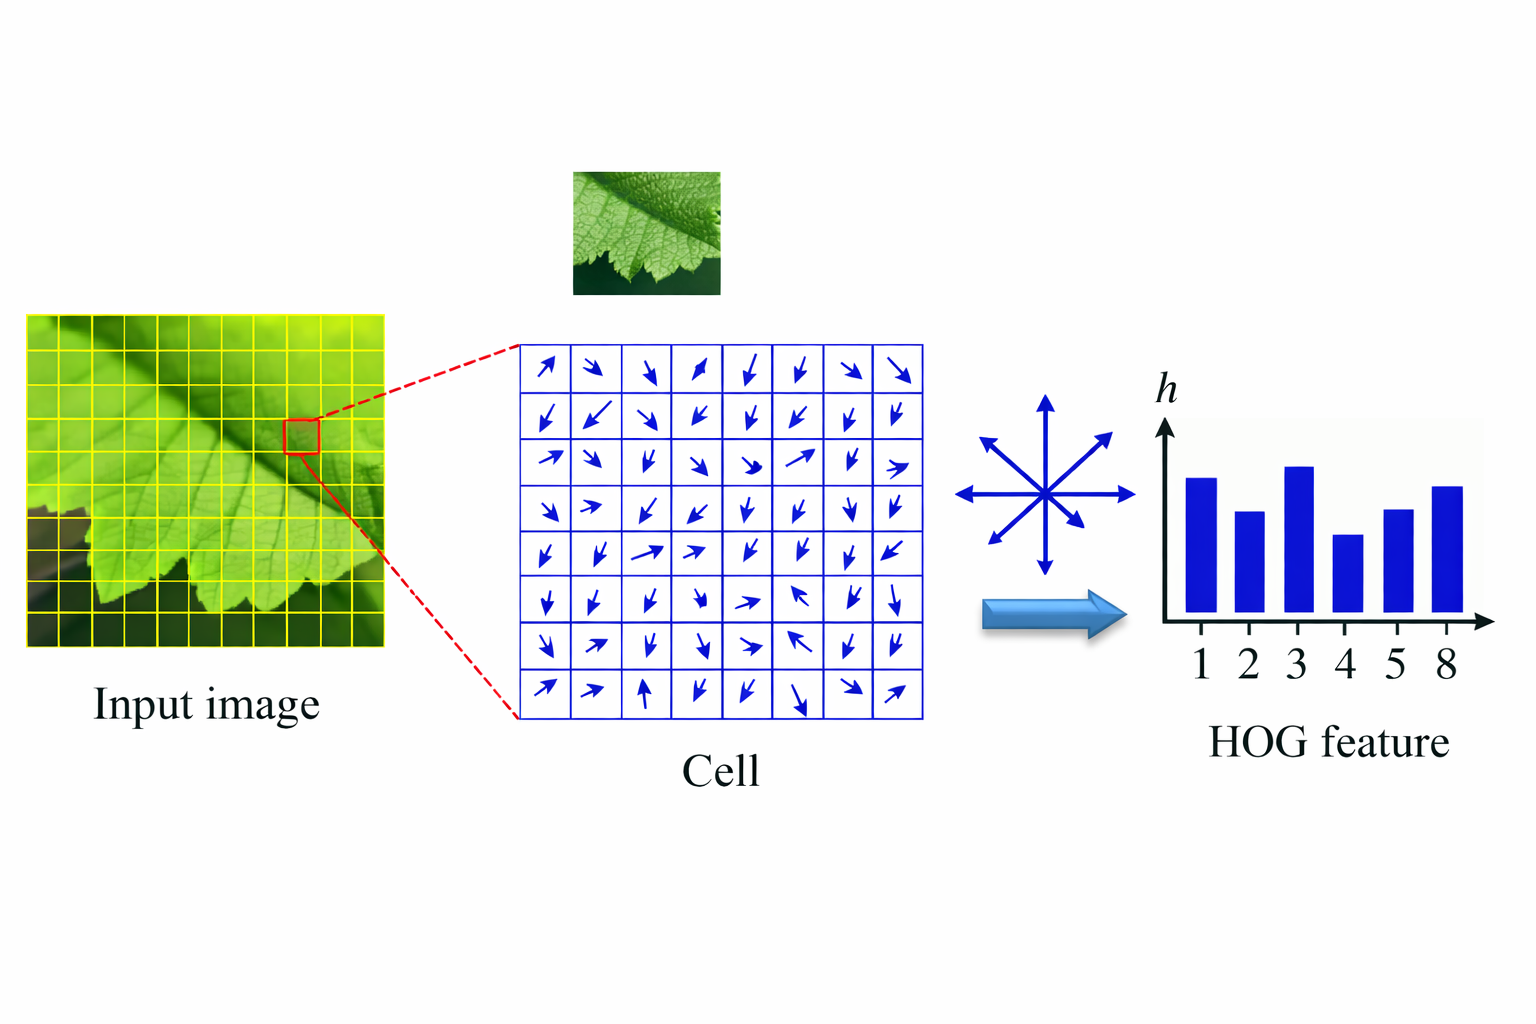
\includegraphics[width=\linewidth]{inc/img/hog_example.png}
	\caption{Иллюстрация получения гистограммы для ячейки}
	\label{hog_example}
\end{figure}
\clearpage

\textbf{Метод k-ближайших соседей}


Метод $k$-ближайших соседей (kNN) является алгоритмом машинного обучения с учителем, первоначально разработанным Эвелин Фикс и Джозефом Ходжесом в 1951 году и впоследствии усовершенствованным Томасом Ковером.

Алгоритм $k$-ближайших соседей (kNN) относится к непараметрическим методам обучения на экземплярах и широко используется в задачах обучения с учителем, включая классификацию и регрессию. В отличие от модельно-ориентированных методов, которые строят явную функцию на основе обучающей выборки, алгоритм kNN относится к классу ленивых алгоритмов обучения. Он не требует предварительного этапа обучения и формирует прогнозы непосредственно при появлении нового объекта, анализируя структуру данных в пространстве признаков. Принцип работы kNN основан на предположении о сходстве данных, согласно которому похожие объекты, как правило, располагаются близко друг к другу в пространстве. Следовательно, прогноз для нового объекта определяется на основе его близости к существующим объектам обучающей выборки.

\textbf{Основные этапы алгоритма kNN.}

\begin{enumerate}
	\item \textbf{Выбор параметра $k$.}  
	На первом этапе выбирается число ближайших соседей $k$, которое является ключевым гиперпараметром алгоритма и подбирается с учётом характеристик конкретного набора данных. Значение $k$ существенно влияет на точность классификации: малые значения $k$ повышают чувствительность к шуму и могут приводить к переобучению, тогда как большие значения $k$ увеличивают вычислительные затраты и могут вызывать недообучение.
	
	\item \textbf{Вычисление расстояний.}  
	Для нового объекта вычисляется расстояние до всех объектов обучающей выборки. Наиболее распространёнными метриками расстояния являются евклидова, манхэттенская и метрика Минковского. Выбор метрики расстояния оказывает значительное влияние на качество работы алгоритма и должен учитывать свойства пространства признаков.
	
	\item \textbf{Определение ближайших соседей.}  
	Все объекты обучающей выборки упорядочиваются по возрастанию расстояния до нового объекта, после чего выбираются $k$ ближайших соседей.
	
	\item \textbf{Агрегация ответов соседей.}  
	В задачах классификации класс нового объекта определяется по принципу большинства голосов среди $k$ ближайших соседей. В задачах регрессии прогнозируемое значение может быть вычислено как среднее или медианное значение целевой переменной соседних объектов.
\end{enumerate}

\textbf{Выбор параметров и его влияние на работу алгоритма:}


Выбор значения $k$ оказывает существенное влияние на поведение модели. Малые значения $k$ могут приводить к переобучению, поскольку алгоритм начинает учитывать шумовые особенности данных. Напротив, большие значения $k$ сглаживают границу принятия решений, что может приводить к потере важной структуры данных и недообучению модели.

Выбор метрики расстояния также является критически важным. Хотя евклидово расстояние используется наиболее часто, альтернативные метрики, такие как манхэттенская или метрика Минковского, могут быть более подходящими при работе с высокоразмерными данными или в случаях, когда требуется различная чувствительность к отдельным признакам.

\textbf{Проблемы алгоритма kNN.}

Современные исследования, посвящённые алгоритму $k$-ближайших соседей, выделяют ряд ключевых проблем.

\begin{enumerate}
	\item Выбор оптимального значения $k$.
	Определение наиболее подходящего числа соседей остаётся сложной задачей, поскольку данный параметр напрямую влияет на точность и обобщающую способность алгоритма.
	
	\item Вычислительная сложность. 
	Классическая реализация kNN требует значительных вычислительных ресурсов при работе с большими наборами данных, так как для каждого нового объекта необходимо вычислять расстояния до всех элементов обучающей выборки.
	
	\item Работа с высокоразмерными данными.
	Эффективность алгоритма kNN снижается в пространствах высокой размерности вследствие эффекта <<проклятия размерности>>, при котором расстояния между объектами теряют информативность.
	
	\item Чувствительность к шуму и выбросам.
	Зависимость алгоритма от ближайших соседей делает его уязвимым к шумовым данным и выбросам, что может негативно сказываться на качестве классификации.
\end{enumerate}

\clearpage

\textbf{Метод опорных векторов}


Метод опорных векторов (Support Vector Machine, SVM) является одним из широко используемых алгоритмов обучения с учителем, применяемых для решения задач классификации и регрессии. В основе метода лежит идея построения оптимальной разделяющей гиперплоскости в пространстве признаков, которая обеспечивает максимальный зазор между объектами различных классов. Такой подход позволяет повысить обобщающую способность классификатора и снизить риск переобучения.

Пусть обучающая выборка задана в виде набора пар $(\mathbf{x}_i, y_i)$, где $\mathbf{x}_i \in \mathbb{R}^d$~---~вектор признаков объекта, а $y_i \in \{-1, +1\}$~---~соответствующая метка класса. В линейно разделимом случае задача SVM заключается в нахождении такой гиперплоскости
\[
\mathbf{w}^T \mathbf{x} + b = 0,
\]
которая разделяет классы и максимизирует расстояние от ближайших объектов обучающей выборки до этой гиперплоскости. Объекты, находящиеся на границе зазора, называются опорными векторами и именно они определяют положение разделяющей поверхности.

Для реальных данных, которые, как правило, не являются строго линейно разделимыми, в методе SVM используется концепция мягкого зазора (soft margin). В этом случае допускаются ошибки классификации, величина которых контролируется с помощью параметра штрафа $C$. Данный параметр задаёт компромисс между шириной зазора и количеством ошибок на обучающей выборке: большие значения $C$ приводят к более строгому разделению классов, тогда как меньшие значения повышают устойчивость модели к шуму.

Для решения задач нелинейной классификации в SVM применяется так называемый ядерный трюк (kernel trick), позволяющий неявно отображать исходные данные в пространство большей размерности, где они могут стать линейно разделимыми. Вместо явного вычисления отображения используется ядерная функция
\[
K(\mathbf{x}_i, \mathbf{x}_j) = \langle \phi(\mathbf{x}_i), \phi(\mathbf{x}_j) \rangle,
\]
которая вычисляет скалярное произведение в новом пространстве признаков. На практике широко применяются линейное, полиномиальное и гауссово (RBF) ядра. Выбор ядра и его параметров существенно влияет на качество классификации и определяется характеристиками конкретной задачи.

Благодаря способности эффективно работать в пространствах высокой размерности и устойчивости к переобучению метод опорных векторов широко используется в задачах анализа изображений, в том числе для классификации объектов на основе заранее извлечённых признаков, таких как LBP и HOG.

\clearpage
